I frequency modulation, FM, vil bærebølgen endre frekvens bestemt av
input signalet.
Når input har høy amplitude får output høyere frekvens.
Når input har lav amplitude blir det lavere frekvens.

\begin{figure}[H]
  \centering
  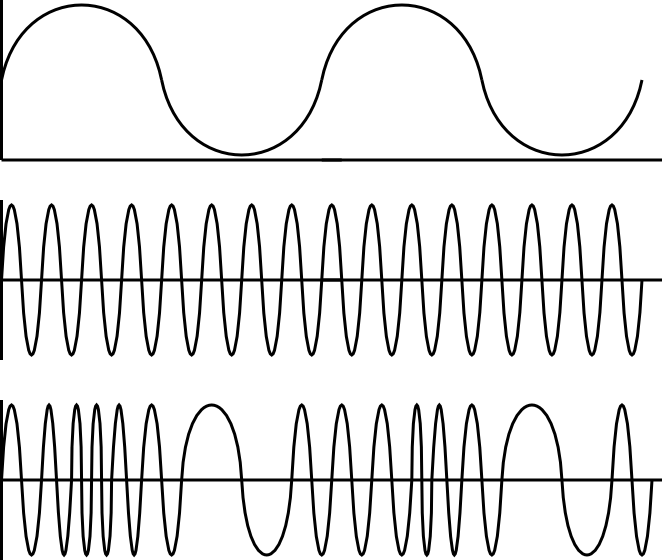
\includegraphics[width=0.67\textwidth]{./img/fm}
  \caption{Output frekvens er raskere der amplituden er høy}
\end{figure}



\paragraph{Problem med stereo} \mbox{} \\
Gamle mottakere var kun kompatible med mono, så når stereo skulle implementeres
i fm ble det problematisk.

Mono-signalet inneholder lyd for høyre og venstre kombinert (L+R).

Løsningen var å bruke en annen kanal til å sende (L-R).
På denne måten kan gamle radioer bruke (L+R), men moderne radioer kan anvende
matematikk på signalene for å hente ut stereo signalene hver for seg.
$$(L+R)+(L-R)=2L$$
$$(L+R)-(L-R)=2R$$

For å sende dette over bare én frekvens brukes tidsmultipleksing (TDM).
Senderen veksler mellom å sende annen hvert signal.
Hvis man veksler med en frekvens på 38kHz kan man reprodusere 15kHz signaler
hos mottaker.
